\chapter*{Mathematical Synthesis}
\addcontentsline{toc}{chapter}{Mathematical Synthesis}

The notes use several models that look different on the surface: perceptrons, receptive fields, membrane equations, phase portraits, cable equations, recurrent networks, and point processes. The common move is always the same. Choose a state, choose an evolution law, choose an observation, and then ask which features of the full biological system survive that projection.

\begin{figure}[h]
\centering
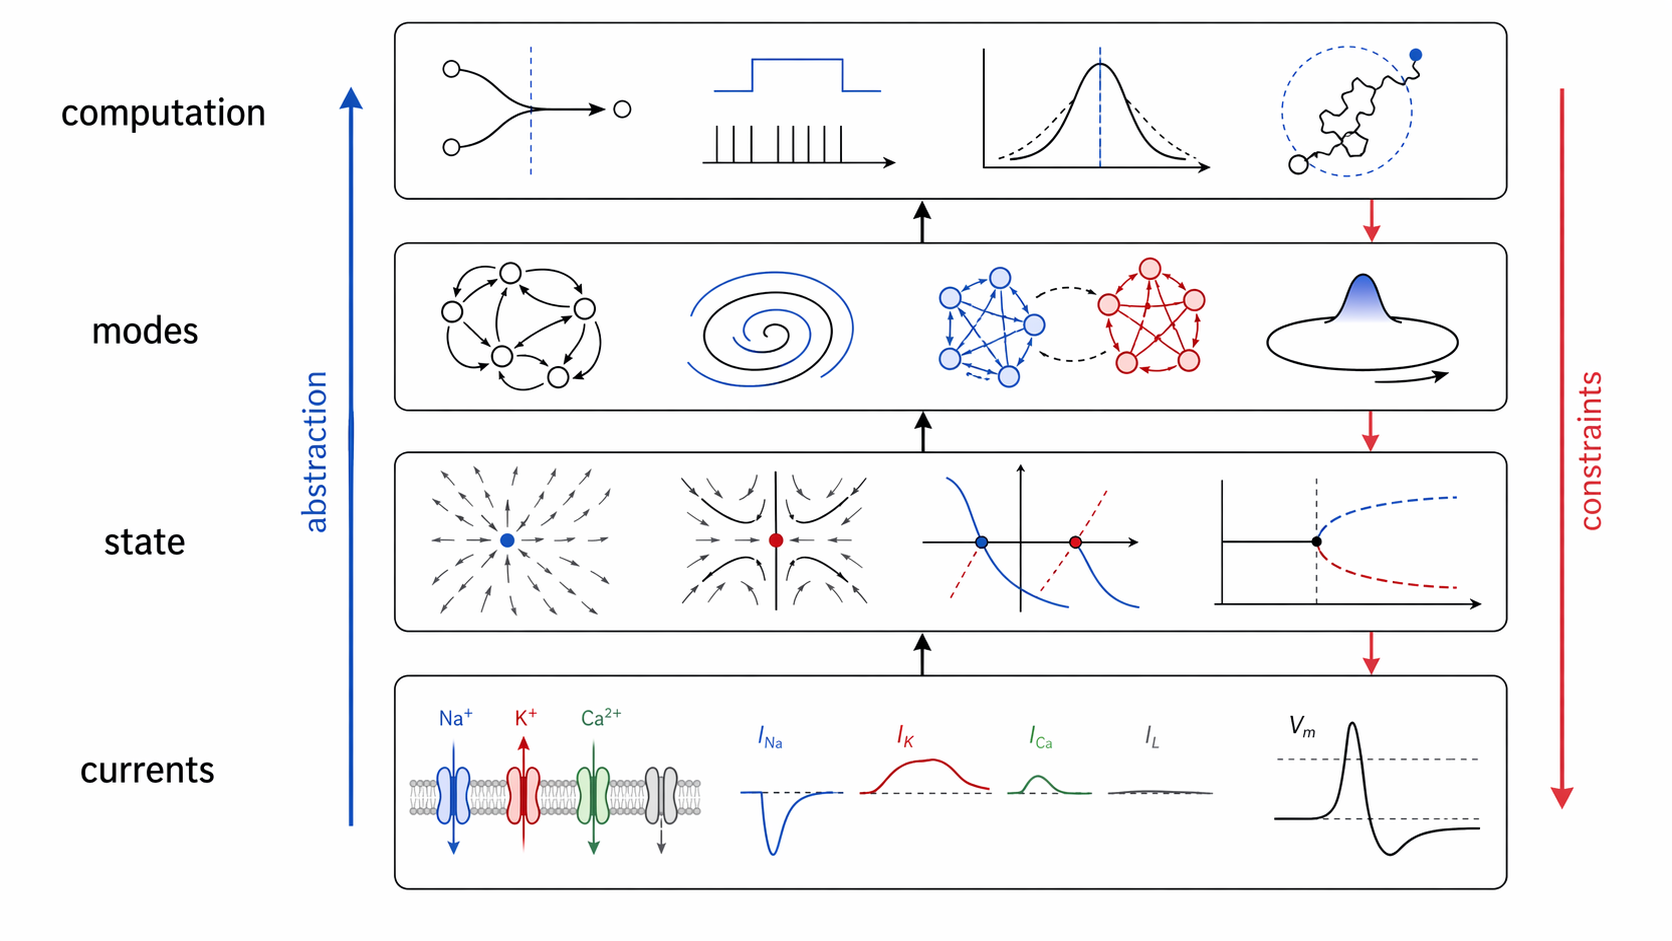
\includegraphics[width=0.96\textwidth]{figures/codex-mns-biophysics-to-computation.png}
\caption{A course-level map from biophysical constraints to computation. Currents determine state dynamics; state dynamics create modes, attractors, and bifurcations; network modes support computations. The downward arrows are just as important: every computational story is constrained by the variables and timescales retained below it.}
\end{figure}

\section*{One Template For Many Models}

A useful neural model usually has the form
\[
  \dot{x} = F(x,u;\theta),
  \qquad
  y = G(x;\theta).
\]
The state \(x\) contains the variables we keep, the input \(u\) contains what is imposed from outside, and the output \(y\) is the quantity we compare with data or behavior. The parameters \(\theta\) collect conductances, time constants, synaptic weights, thresholds, and noise scales.

The art is not to make \(x\) large. The art is to make \(x\) honest. If the question is spike onset, \(x=(V,n)\) may be enough to expose a threshold geometry. If the question is propagation along a dendrite, \(x\) becomes a voltage field \(V(x,t)\). If the question is memory or selection, \(x\) may be a population activity vector.

\begin{aside}[Minimality principle]
A model is good when the variables it removes are genuinely irrelevant to the question. It is bad when the variables it removes are the hidden mechanism.
\end{aside}

\section*{Biophysics As A Constraint}

The membrane equation is the cleanest example of how physical accounting becomes dynamics:
\[
  C_m \frac{dV}{dt}
  =
  -\sum_k g_k(V,t)\bigl(V-E_k\bigr) + I_{\mathrm{ext}}(t).
\]
Every current is a product of a conductance and a driving force. The reversal potential \(E_k\) says where the current would vanish; the conductance \(g_k\) says how strongly the channel population can move the voltage toward that value.

This is why the same equation can support several levels of explanation. If \(g_k\) is constant, the cell is a leaky integrator. If \(g_k\) depends on gating variables, the cell can spike. If the voltage is spread over space, the same current balance becomes a cable equation. The mathematical structure changes slowly; the interpretation of the state changes sharply.

\section*{Geometry Near A State}

Around a fixed point \(x^\ast\), nonlinear dynamics have a local linear approximation
\[
  \delta \dot{x}
  =
  J(x^\ast)\,\delta x,
  \qquad
  J_{ij}(x^\ast)=\pd{F_i}{x_j}(x^\ast).
\]
The eigenvalues of \(J\) are a local grammar for behavior. Negative real parts pull trajectories inward. Positive real parts push them away. Complex eigenvalues introduce rotation. A bifurcation occurs when parameter changes move this local grammar through a qualitative boundary, for example when a stable rest state collides with an unstable threshold or when a spiral loses stability.

This viewpoint unifies phase-plane analysis and recurrent-network analysis. In a two-variable neuron model, the eigenvectors describe local motion near a fixed point. In a recurrent population model, eigenvectors describe modes of population activity. Stability, amplification, memory, and oscillation all become statements about the spectrum of a linearized operator.

\section*{Noise As A Model Component}

Variability is not merely measurement error. Channel openings, synaptic release, and spike timing all introduce randomness that can matter for computation. A point-process description makes this explicit:
\[
  \lambda(t \mid \mathcal{H}_t)
  =
  \phi\!\left(b + k^\top s(t) + h^\top \rho_{<t}\right),
\]
where \(\lambda\) is the conditional intensity, \(s(t)\) is the stimulus history, and \(\rho_{<t}\) is the recent spike history. The deterministic part says what drives the cell; the stochastic part says how that drive is expressed in finite spike trains.

The central lesson is that neural systems are not either biophysical or computational. They are computational because biophysics creates reproducible state transformations, and they are biophysical because every computation must be implemented by currents, timescales, geometry, and noise.
